\section{实验结果与分析}
% 一些关于序号的设置
\setcounter{figure}{0}

\subsection{改进SSD算法的实验结果}
\begin{uscfigure}
	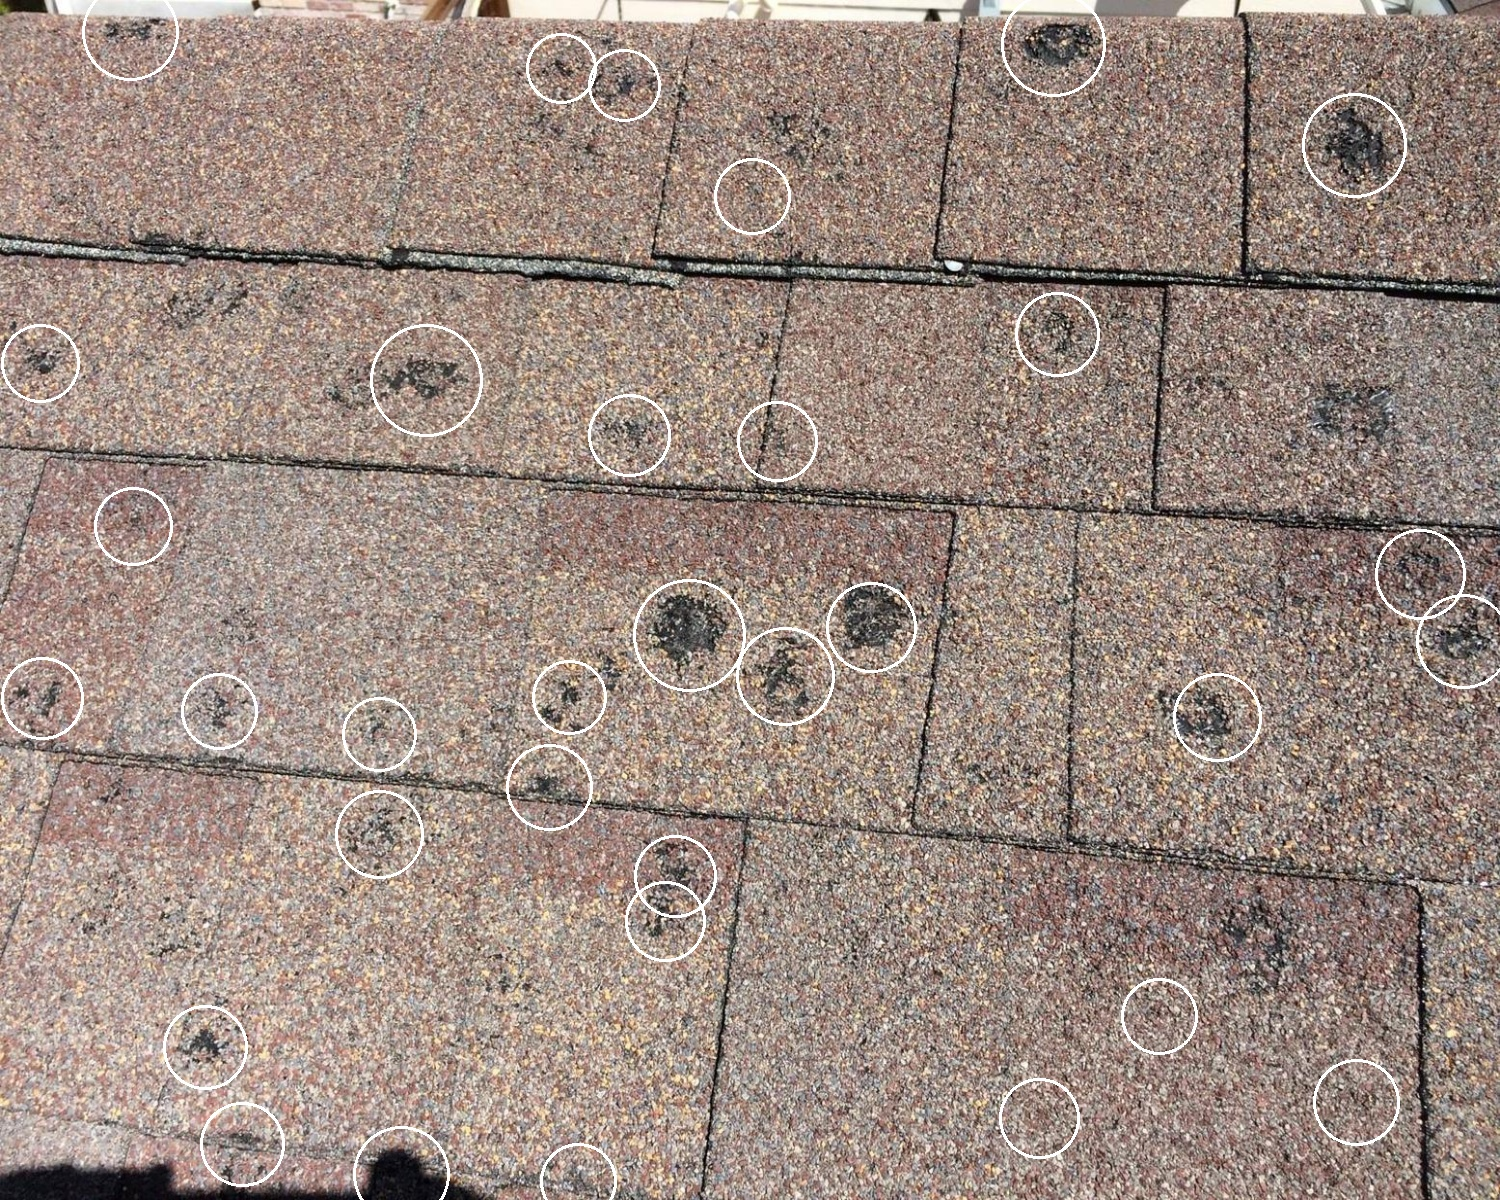
\includegraphics[width=\textwidth]{./Pictures/result.jpg}	
	\caption{检测结果}
	\label{result}
\end{uscfigure}
\subsection{改进SSD对瓦片损害检测的准确率实验}
\begin{table}[htbp]
	\centering
	\caption{改进SSD算法的准确率实验结果}
	\label{}
	\begin{tabular}{ccc}
		\toprule
		网络模型 & mAP & fps\\
		\midrule
		SSD 	& 75\% & 60\\
		改进SSD  &  60\% & 50\\
		\bottomrule
	\end{tabular}
\end{table}
\subsection{SSD 与修改了focus loss 的算法进行mAP、速度的比较}
\begin{table}[htbp]
	\centering
	\caption{改进SSD算法的准确率实验结果}
	\label{}
	\begin{tabular}{ccc}
		\toprule
		网络模型 & mAP & fps\\
		\midrule
		SSD 	& 75\% & 60\\
		SSD+focus loss  &  60\% & 50\\
		\bottomrule
	\end{tabular}
\end{table}

